
\chapter{Specifikacija programske potpore}

\section{Funkcionalni zahtjevi}

\noindent \textbf{Dionici:}

\begin{packed_enum}
	
	\item Donor		
	\item Djelatnik banke	
	\item Administrator
	\item Razvojni tim
	
\end{packed_enum}

\noindent \textbf{Aktori i njihovi funkcionalni zahtjevi:}


\begin{packed_enum}
	\item  \underbar{Neregistrirani/neprijavljeni korisnik(inicijator) može:}
	
	\begin{packed_enum}
		
		\item pregledati trenutno stanje zaliha
		\item se registrirati u sustav, stvoriti korisnički račun za koji su mu potrebni matični i kontakt podaci
		
	\end{packed_enum}
	
	\item  \underbar{Donor (inicijator) može:}
	
	\begin{packed_enum}
		
		\item pregledavati i mijenjati osobne podatke
		\item pregledavati povijest svojih doniranja
		\item iz aplikacije dobiti PDF potvrdu
		\item pregledati poruku u ovisnosti o trenutnom stanju zaliha krvi
		
	\end{packed_enum}
	
	\item  \underbar{Djelatnik banke (inicijator) može:}
	
	\begin{packed_enum}
		
		\item kreirati korisnički profil donora
		\item evidentirati svaki pokušaj doniranja (uspješan / neuspješan) 
		\item evidentirati privremeno ili trajno odbijanje
		\item evidentirati potrošnju krvi 
		\item aktivirati račun aktivacijskim linkom i odabrati lozinku
		\item vidjeti popis registriranih donora
		
	\end{packed_enum}
	\eject
	
	\item  \underbar{Administrator (inicijator) može:}
	
	\begin{packed_enum}
		
		\item definirati gornju i donju granicu optimalne količine krvi
		\item kreirati nove korisničke račune za ulogu djelatnika banke
		\item deaktivirati korisnički račun djelatnika banke ili donora
		\item vidjeti popis registriranih svih korisnika i njihovih osobnih podataka
		
	\end{packed_enum}
	
	\item  \underbar{Baza podataka (sudionik):}
	
	\begin{packed_enum}
		
		\item pohranjuje sve podatke o korisnicima i njihovim ovlastima
		\item pohranjuje trenutno stanje količine krvi,te donju i gornju granicu optimalne količine krvi
		
	\end{packed_enum}
	
	\item  \underbar{Sustav za automatske poslove(inicijator) može:}
	
	\begin{packed_enum}
		
		\item slati email notifikacije donoru nakon 3 mjeseca od uspješnog darivanja ako je muškarac ili nakon 4 mjeseca ako je žensko
		\item slati email notifikacije donoru i djelatniku banke ako se pređu granice određene krve grupe
		
	\end{packed_enum}
\end{packed_enum}



\eject 



\subsection{Obrasci uporabe}

\subsubsection{Opis obrazaca uporabe}


\noindent \underbar{\textbf{UC1 - Pregled količine krvi}}
					\begin{packed_item}
	
						\item \textbf{Glavni sudionik: }Korisnik, Donor, Djelatnik banke, Administrator
						\item \textbf{Cilj:} Prikazati trenutnu količinu krvi u banci
						\item \textbf{Sudionici:} Baza podataka
						\item \textbf{Preduvjet:} -
						\item \textbf{Opis osnovnog tijeka:}
						
						\item[] \begin{packed_enum}
	
							\item Količine krvi su prikazane otvaranjem aplikacije, te njihove gornje i donje granice
							
						\end{packed_enum}

					\end{packed_item}

\noindent \underbar{\textbf{UC2 - Registracija}}
					\begin{packed_item}
	
						\item \textbf{Glavni sudionik: }Korisnik, djelatnik banke
						\item \textbf{Cilj:} Stvoriti korisnički račun donora za pristup sustavu
						\item \textbf{Sudionici:} Baza podataka
						\item \textbf{Preduvjet:} -
						\item \textbf{Opis osnovnog tijeka:}
						
						\item[] \begin{packed_enum}
	
							\item Korisnik/Djelatnik banke odabire opciju za registraciju novog donora
							\item Korisnik/Djelatnik banke unosi potrebne podatke
							\item Korisnik/Donor na svoj mail dobiva aktivacijski link
							
						\end{packed_enum}
						
						\item  \textbf{Opis mogućih odstupanja:}
						
						\item[] \begin{packed_item}
	
							\item[2.a] Odabir već korištenog e-maila, unos podataka u nedozvoljenom formatu ili unos neispravnog e-maila
							\item[] \begin{packed_enum}
								
								\item Korisnik dobiva obavijest o neuspjelom upisu i vraća ga na stranicu za registraciju
								\item Korisnik mijenja potrebne podatke ili odustaje od registracije
								
							\end{packed_enum}
							
							
						\end{packed_item}
					\end{packed_item}
\eject 
\noindent \underbar{\textbf{UC3 - Prijava u sustav}}
					\begin{packed_item}
	
						\item \textbf{Glavni sudionik: }Donor, djelatnik
						\item \textbf{Cilj:} Prijava u sustav i dobivanje dodatnih mogućnosti aplikacije
						\item \textbf{Sudionici:} Baza podataka
						\item \textbf{Preduvjet:} Registracija
						\item \textbf{Opis osnovnog tijeka:}
						
						\item[] \begin{packed_enum}
	
							\item Unos e-maila i lozinke
							\item Potvrda ispravnosti unesenih podataka
							\item Pristup dodatnim mogućnostima
							
						\end{packed_enum}
						\item  \textbf{Opis mogućih odstupanja:}
						
						\item[] \begin{packed_item}
	
							\item[2.a] Neispravan e-mail i/ili lozinka
							\item[] \begin{packed_enum}
								
								\item  Sustav obavještava korisnika o neuspjeloj prijavi i vraća ga na stranicu za prijavu

								
							\end{packed_enum}
					\end{packed_item}
					\end{packed_item}
\noindent \underbar{\textbf{UC4 - Pregled osobnih podataka}}
					\begin{packed_item}
	
						\item \textbf{Glavni sudionik: }Donor
						\item \textbf{Cilj:} Prikazati osobne podatke prijavljenog donora
						\item \textbf{Sudionici:} Baza podataka
						\item \textbf{Preduvjet:} Donor je prijavljen
						\item \textbf{Opis osnovnog tijeka:}
						
						\item[] \begin{packed_enum}
	
							\item Donor odabire opciju "Osobni podaci"
							\item Aplikacija prikazuje osobne podatke donora
							
						\end{packed_enum}

					\end{packed_item}
\eject 
\noindent \underbar{\textbf{UC5 - Promjena matičnih i/ili kontakt podataka}}
					\begin{packed_item}
	
						\item \textbf{Glavni sudionik: }Donor
						\item \textbf{Cilj:} Promjeniti matične i/ili kotakt podatke
						\item \textbf{Sudionici:} Baza podataka
						\item \textbf{Preduvjet:} Donor je prijavljen
						\item \textbf{Opis osnovnog tijeka:}
						
						\item[] \begin{packed_enum}
	
							\item Donor odabire opciju "Promijeni osobne podatka"
							\item Donor mijenja svoje podatke
							\item Donor sprema promjene
							\item Ažurira se baza podataka
							
						\end{packed_enum}

						\item  \textbf{Opis mogućih odstupanja:}
						
						\item[] \begin{packed_item}
	
							\item[2.a] Korisnik ne spremi promjenu
							\item[] \begin{packed_enum}
								
								\item  Sustav obavještava korisnika da nije spremio podatke prilikom izlaska iz prozora

								
									\end{packed_enum}
								\end{packed_item}
					\end{packed_item}
\noindent \underbar{\textbf{UC6 - Pregled povijesti darivanja}}
					\begin{packed_item}
	
						\item \textbf{Glavni sudionik: }Donor
						\item \textbf{Cilj:} Pregledati svoju povijest darivanja krvi
						\item \textbf{Sudionici:} Baza podataka
						\item \textbf{Preduvjet:} Donor je prijavljen
						\item \textbf{Opis osnovnog tijeka:}
						
						\item[] \begin{packed_enum}
	
							\item Donor odabire opciju "Povijest darivanja"
							\item aplikacija prikazuje donorovu povijest darivanja
							
						\end{packed_enum}

					\end{packed_item}
\eject 
\noindent \underbar{\textbf{UC7 - Dobivanje PDF potvrde o doniranju}}
					\begin{packed_item}
	
						\item \textbf{Glavni sudionik: }Donor
						\item \textbf{Cilj:} Dobiti PDF potvrdu o doniranju
						\item \textbf{Sudionici:} Baza podataka
						\item \textbf{Preduvjet:} Donor je prijavljen i barem jedanput uspješno darovao krv
						\item \textbf{Opis osnovnog tijeka:}
						
						\item[] \begin{packed_enum}
	
							\item Donor odabire opciju "Povijest darivanja"
							\item Donor odabire opciju "Želim PDF potvrdu"
							\item Sustav donoru šalje potvrdu na mail
							
						\end{packed_enum}

					\end{packed_item}

\noindent \underbar{\textbf{UC8 - Dobivanje poruke stanja zalihe krvi}}
					\begin{packed_item}
	
						\item \textbf{Glavni sudionik: }Donor
						\item \textbf{Cilj:} dobiti poruku stanja zaliha krvi
						\item \textbf{Sudionici:} Baza podataka
						\item \textbf{Preduvjet:} Donor je prijavljen i nema trajnu zabranu darivanja krvi
						\item \textbf{Opis osnovnog tijeka:}
						
						\item[] \begin{packed_enum}
	
							\item Donor se prijavio u sustav
							\item Donor dobiva poruku o ovisnosti stanja zaliha krvi
							
						\end{packed_enum}

					\end{packed_item}


\noindent \underbar{\textbf{UC9 - Evidentiranje "potrošnje" krvi}}
					\begin{packed_item}
	
						\item \textbf{Glavni sudionik: }Djelatnik
						\item \textbf{Cilj:} slanje određenog broja jedinica krvi u vanjsku instituciju
						\item \textbf{Sudionici:} Baza podataka
						\item \textbf{Preduvjet:} Djelatnik je prijavljen
						\item \textbf{Opis osnovnog tijeka:}
						
						\item[] \begin{packed_enum}
	
							\item Djelatnik odabire krvnu grupu čiju zalihu želi evidentirati
							\item Djelatnik upisuje količinu
							\item Djelatnik šalje krv u vanjsku instituciju
						\end{packed_enum}
						\item  \textbf{Opis mogućih odstupanja:}
						
						\item[] \begin{packed_item}
	
							\item[2.a] Količina krvi iznosi 0
							\item[] \begin{packed_enum}
								
								\item  Sustav obavještava djelatnika da ne može poslati krv vanjskoj jedinici

								
							\end{packed_enum}
					\end{packed_item}
					\end{packed_item}

\eject 
\noindent \underbar{\textbf{UC10 - Pregled popisa registriranih donora}}
					\begin{packed_item}
	
						\item \textbf{Glavni sudionik: }Djelatnik
						\item \textbf{Cilj:} Prikazati popis svih registriranih donora
						\item \textbf{Sudionici:} Baza podataka
						\item \textbf{Preduvjet:} Djelatnik je prijavljen
						\item \textbf{Opis osnovnog tijeka:}
						
						\item[] \begin{packed_enum}
	
							\item Djelatnik odabire opciju "Popis donora"
							\item Sustav djelatniku prikazuje popis registriranih donora
						\end{packed_enum}

					\end{packed_item}


\noindent \underbar{\textbf{UC$11$ -{Aktivacija računa}	}}
\begin{packed_item}
	
	\item \textbf{Glavni sudionik: } {Korisnik, djelatnik banke}
	\item  \textbf{Cilj:} {Aktivirati račun}
	\item  \textbf{Sudionici:}{Baza podataka} 
	\item  \textbf{Preduvjet:}{Registracija}
	\item  \textbf{Opis osnovnog tijeka:}
	
	\item[] \begin{packed_enum}
		
		\item {Korisnika nakon klika na link u mailu vodi u aplikaciju}
		\item {Prikazuje se poruka o uspješnoj registraciji i traži se odabir lozinke} 
		\item {Korisnik odabire lozinku}
		\item {Korisnik se automatski prijavljuje}
		
	\end{packed_enum}
	
\end{packed_item}

\noindent \underbar{\textbf{UC$12$ -{Evidentiranje pokušaja doniranja}	}}
\begin{packed_item}
	
	\item \textbf{Glavni sudionik: }{Djelatnik banke}
	\item  \textbf{Cilj:} {Evidentirati pokušaj doniranja}
	\item  \textbf{Sudionici:}{Baza podataka} 
	\item  \textbf{Preduvjet:}{Registracija}
	\item  \textbf{Opis osnovnog tijeka:}
	
	\item[] \begin{packed_enum}
		
		\item {Djelatnik odabere opciju za evidentiranje pokušaja doniranja određenog donora}
		\item {Djelatnik evidentira s uspješan ili neuspješan pokušaj}
		\item {Djelatnik banke sprema promjene}
		\item {Baza podataka se ažurira, povećava se razina određene vrste krvi i zapisuje se pokušaj doniranja krvi}
		\item {Sustav šalje email poruku s PDF potvrdom}
		
	\end{packed_enum}
	
\end{packed_item}
\eject 
\noindent \underbar{\textbf{UC$13$ -{Brisanje donora}	}}
\begin{packed_item}
	
	\item \textbf{Glavni sudionik: }{Administrator}
	\item  \textbf{Cilj:} {Izbrisati kor. račun donora}
	\item  \textbf{Sudionici:}{Baza podataka}
	\item  \textbf{Preduvjet:}{Administrator prijavljen}
	\item  \textbf{Opis osnovnog tijeka:}
	
	\item[] \begin{packed_enum}
		
		\item {Administrator odabire opciju Prikaz donora}
		\item {Administratoru se pokažu registrirani donori} 
		\item {Administrator briše donora}
		
	\end{packed_enum}
	
\end{packed_item}

\noindent \underbar{\textbf{UC$14$ -{Definiranje optimalnih granica}	}}
\begin{packed_item}
	
	\item \textbf{Glavni sudionik: }{Administrator}
	\item  \textbf{Cilj:} {Definirati gornju i donju granicu optimalnih količina krvi za pojedinu grupu}
	\item  \textbf{Sudionici:}{Baza podataka}
	\item  \textbf{Preduvjet:}{Administrator je prijavljen}
	\item  \textbf{Opis osnovnog tijeka:}
	
	\item[] \begin{packed_enum}
		
		\item {Administrator odabire opciju "Definiraj granice"}
		\item {Prikazuju se trenutno određene granice za pojedinu vrstu krvi} 
		\item {Administrator definira granice za pojedinu vrstu krvi}
		\item {Administrator sprema promjene}
		
	\end{packed_enum}
\end{packed_item}

\noindent \underbar{\textbf{UC$15$ -{Pregled popisa djelatnika}	}}
\begin{packed_item}
	
	\item \textbf{Glavni sudionik: }{Administartor}
	\item  \textbf{Cilj:} {Prikazati popis svih djelatnika banke}
	\item  \textbf{Sudionici:}{Baza podataka} 
	\item  \textbf{Preduvjet:}{Administrator je prijavljen}
	\item  \textbf{Opis osnovnog tijeka:}
	
	\item[] \begin{packed_enum}
		
		\item {Administrator odabire opciju "Prikaz popisa djelatnika banke"}
		\item {Prikazuje se popis svih djelatnika banke po abecednom redu}
		\end{packed_enum}
\end{packed_item}

\eject 
\noindent \underbar{\textbf{UC$16$ -{Brisanje djelatnika banke}	}}
\begin{packed_item}
	
	\item \textbf{Glavni sudionik: }{Administrator}
	\item  \textbf{Cilj:} {Izbrisati kor. račun djelatnika banke}
	\item  \textbf{Sudionici:}{Baza podataka}
	\item  \textbf{Preduvjet:}{Administrator prijavljen}
	\item  \textbf{Opis osnovnog tijeka:}
	
	\item[] \begin{packed_enum}
		
		\item {Administrator odabire opciju Prikaz djelatnika banke}
		\item {Administratoru se pokažu registrirani djelatnici banke}
		\item {Administrator briše djelatnika banke}
		
	\end{packed_enum}
	
\end{packed_item}

\noindent \underbar{\textbf{UC$17$ -{Kreiranje kor. računa djelatnika banke}	}}
\begin{packed_item}
	
	\item \textbf{Glavni sudionik: }{Administrator}
	\item  \textbf{Cilj:} {Kreirati računa djelatnika banke}
	\item  \textbf{Sudionici:}{Baza podataka}
	\item  \textbf{Preduvjet:}{Administrator je prijavljen}
	\item  \textbf{Opis osnovnog tijeka:}
	
	\item[] \begin{packed_enum}
		
		\item {Administrator odabire opciju "Kreiraj korisnički račun djelatnika banke"}
		\item {Prikazuje se forma koju popunjava} 
		\item {Odabire opciju "Kreiraj račun"}
		\item {Baza podataka se ažurira}
		\item {Šalje se aktivacijski link na email djelatnika banke}
	\end{packed_enum}
	
	\item  \textbf{Opis mogućih odstupanja:}
	
	\item[] \begin{packed_item}
		
		\item[2.a] $<$opis mogućeg scenarija odstupanja u koraku 2$>$
		\item[] \begin{packed_enum}
			
			\item $<$opis rješenja mogućeg scenarija korak 1$>$
			\item $<$opis rješenja mogućeg scenarija korak 2$>$
			
		\end{packed_enum}
		\item[2.b] $<$opis mogućeg scenarija odstupanja u koraku 2$>$
		\item[3.a] $<$opis mogućeg scenarija odstupanja  u koraku 3$>$
		
	\end{packed_item}
\end{packed_item}
\eject 
\noindent \underbar{\textbf{UC$18$ -{Slanje notifikacije nakon 3/4 mjeseca}	}}
\begin{packed_item}
	
	\item \textbf{Glavni sudionik: }{Sustav za automatske poslove}
	\item  \textbf{Cilj:} {Poslati notifikaciju donoru}
	\item  \textbf{Sudionici:}{Baza podataka}
	\item  \textbf{Preduvjet:}{Prošlo 3 mjeseca od uspješnog darivanja}
	\item  \textbf{Opis osnovnog tijeka:}
	
	\item[] \begin{packed_enum}
		
		\item {Sustav svakodnevno provjerava uspješna doniranja od prije 3 mjeseca za muškarce i od prije 4 mjeseca za žene}
		\item {Svima koji zadovoljavaju uvjet šalju se email notifikacije da mogu doći ponovno donirati krv}
		
	\end{packed_enum}
	
\end{packed_item}

\noindent \underbar{\textbf{UC$19$ -{Slanje notifikacije ako se prijeđu granice}	}}
\begin{packed_item}
	
	\item \textbf{Glavni sudionik: }{Sustav za automatske poslove}
	\item  \textbf{Cilj:} {Poslati notifikaciju donoru i djelatniku banke}
	\item  \textbf{Sudionici:}{Baza podataka}
	\item  \textbf{Preduvjet:}{Prešle su se optimalne granice}
	\item  \textbf{Opis osnovnog tijeka:}
	
	\item[] \begin{packed_enum}
		
		\item {Ako je došlo do prekoračenja gornje granice šalje se notifikacija na email djelatnika banke}
		\item {Ako je došlo do pada ispod donje granice šalje se notifikacija na email donora ako je te krvne grupe i djelatniku banke}
		
		
	\end{packed_enum}
	
\end{packed_item}

\subsubsection{Dijagrami obrazaca uporabe}
\begin{figure}[H]
			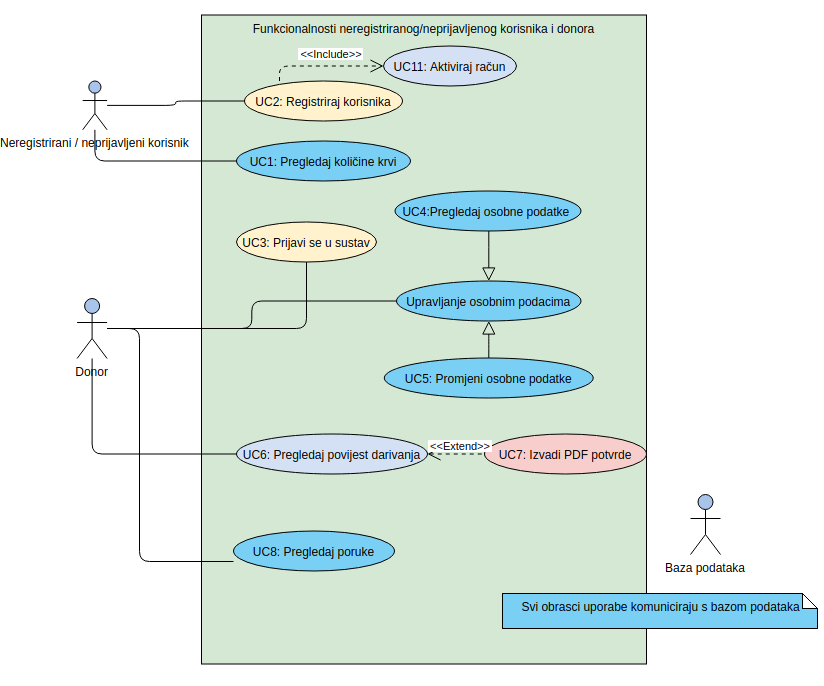
\includegraphics[scale=0.6]{dijagrami/Funkcionalnosti_korisnika_donora.png} %veličina slike u odnosu na originalnu datoteku i pozicija slike
			\centering
			\caption{Dijagram obrasca uporabe, funkcionalnost korisnika i donora}
			\label{fig:Funkcionalnosti_korisnika_donora}
\end{figure}

\begin{figure}[H]
			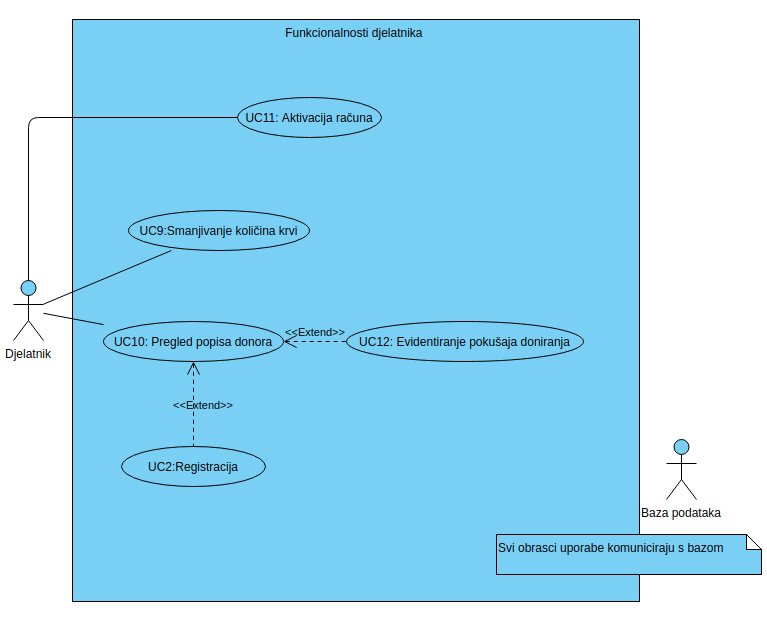
\includegraphics[scale=0.6]{dijagrami/Funkcionalnosti_djelatnika_donora.png} %veličina slike u odnosu na originalnu datoteku i pozicija slike
			\centering
			\caption{Dijagram obrasca uporabe, funkcionalnost djelatnika i donora}
			\label{fig:Funkcionalnosti_djelatnika_donora}
\end{figure}

\begin{figure}[H]
			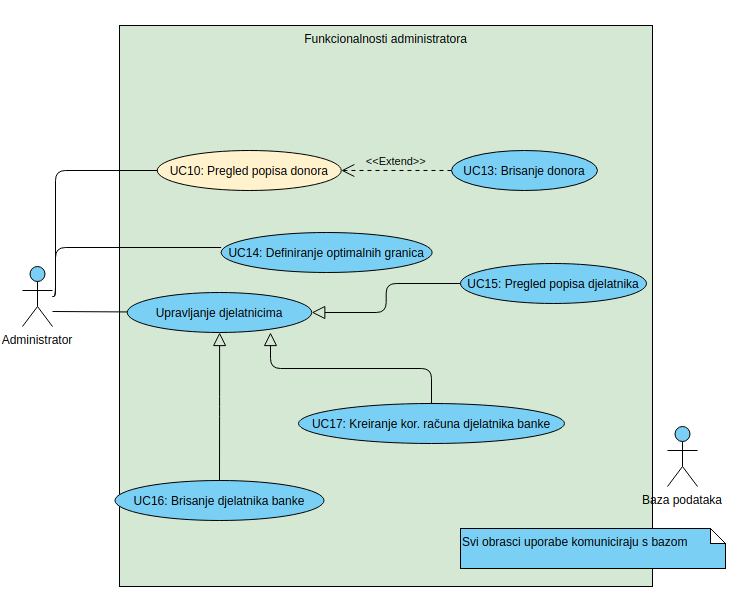
\includegraphics[scale=0.6]{dijagrami/Funkcionalnosti_admina.png} %veličina slike u odnosu na originalnu datoteku i pozicija slike
			\centering
			\caption{Dijagram obrasca uporabe, funkcionalnost administratora}
			\label{fig:Funkcionalnosti_admina}
\end{figure}

\begin{figure}[H]
			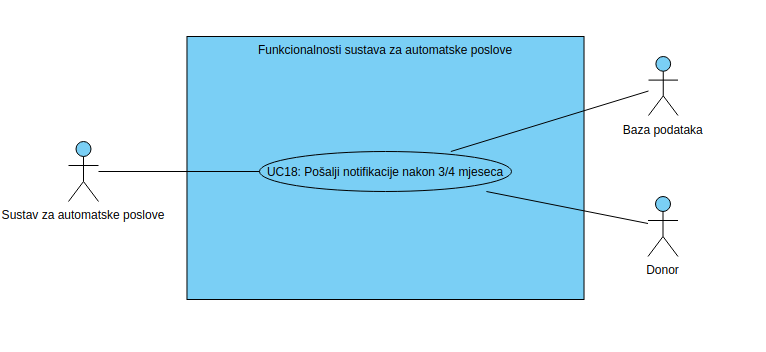
\includegraphics[scale=0.6]{dijagrami/Funkcionalnosti_auto.png} %veličina slike u odnosu na originalnu datoteku i pozicija slike
			\centering
			\caption{Dijagram obrasca uporabe, funkcionalnost sustava za automatske poslove}
			\label{fig:Funkcionalnosti_auto}
\end{figure}

\eject
		
\subsection{Sekvencijski dijagrami}

\textbf{Obrazac uporabe UC8 - Dobivanje poruke stanja zalihe krvi}

Donor, koji nema trajnu zabranu darivanja krvi, kod svakog spajanja u sustav dobiva poruku u ovisnosti o trenutnom stanju zaliha krvi. Poslužitelj dohvaća podatke iz baze podataka i prema zadanim granicama vraća jednu od tri poruka. Poruke mogu biti: stanje zaliha ispod optimalne granice; stanje zaliha je optimalno; stanje zaliha je iznad gornje optimalne granice.

\begin{figure}[H]
	\centering
	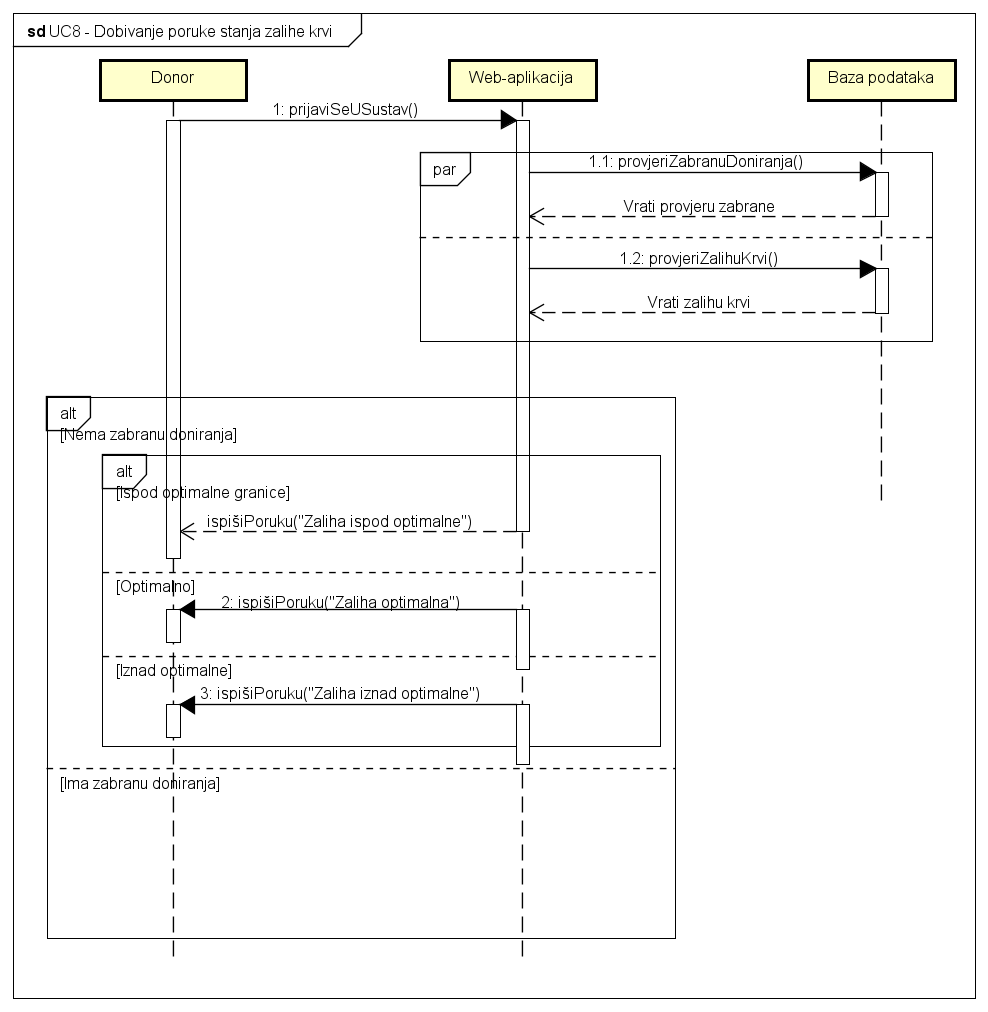
\includegraphics[width=\textwidth, scale=0.4]{dijagrami/UC8_Dobivanje poruke stanja zalihe krvi.png}
	\caption{Sekvencijski dijagram za UC8}
	\label{fig:UC8_Dobivanje poruke stanja zalihe krvi}
\end{figure}
\eject

\textbf{Obrazac uporabe UC9 - Evidentiranje "potrošnje" krvi}

Djelatnik banke može evidentirati "potrošnju" krvi odnosno slanje određenog broja jedinica krvi u vanjsku instituciju. U bazi podataka se smanjuje količina određene vrste krvi.

\begin{figure}[H]
	\centering
	\includegraphics[width=\textwidth, scale=0.4]{dijagrami/UC9_Evidentiranje_potrošnje_ krvi.png}
	\caption{Sekvencijski dijagram za UC9}
\end{figure}

\eject 
\textbf{Obrazac uporabe UC12 - Evidentiranje pokušaja doniranja}

Djelatnik banke evidentira i uspješne i neuspješne pokušaje doniranja. Na temelju zdravstvenog stanja donor može pristupiti doniranju, ali može i biti privremeno ili trajno odbijen. Baza podataka se ažurira, zapisuje se pokušaj doniranja krvi i ako je uspješan poveća se razina određene vrste krvi.

\begin{figure}[H]
	\centering
	\includegraphics[width=\textwidth]{dijagrami/UC12_Evidentiranje pokušaja doniranja.png}
	\caption{Sekvencijski dijagram za UC12}
\end{figure}
\eject

\textbf{Obrazac uporabe UC14 - Definiranje optimalnih granica}

Za svaku krvnu grupu administrator sustava definira gornju i donju granicu optimalne količine. Administratoru se prikazuju trenutne granice za pojedinu vrstu krvi. Zatim on ih on može mijenjati i promjene se spremaju i bazu podataka.

\begin{figure}[H]
	\centering
	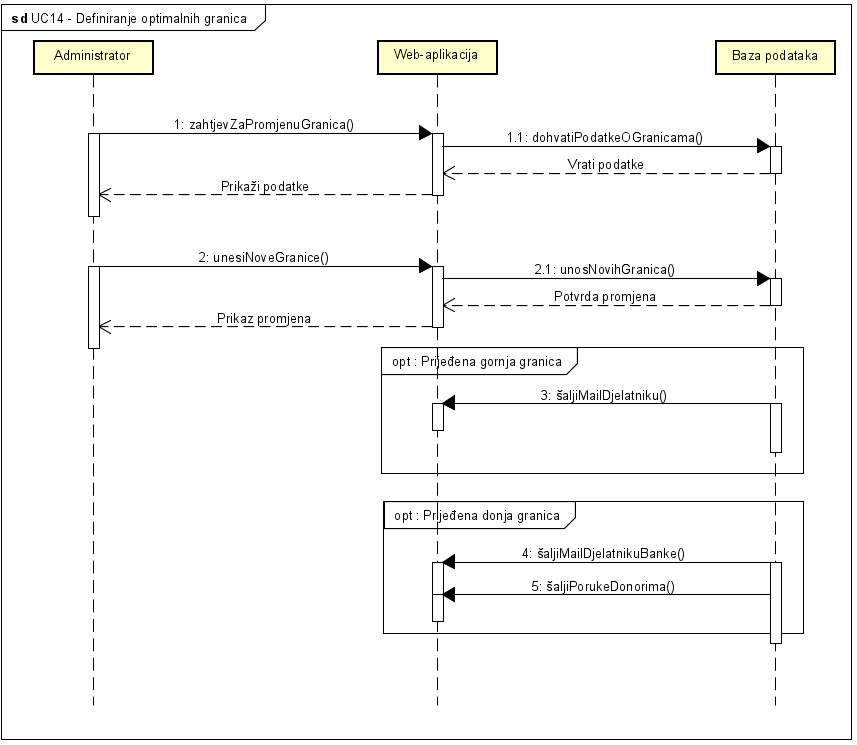
\includegraphics[width=\textwidth]{dijagrami/UC14_Definiranje optimalnih granica.png}
	\caption{Sekvencijski dijagram za UC14}
\end{figure}
\eject

\section{Ostali zahtjevi}

\begin{packed_item}
	
	\item Sustav treba biti implementiran kao web aplikacija koja je prilagođena različitim veličinama ekrana. (responsive web design)
	\item Sustavu trebaju moći pristupati tri vrste korisnika (administrator, djelatnik banke i donor). Svaki korisnik se treba ovjeravati korisničkim imenom i lozinkom.
	\item Treba postojati javna web stranica koja prikazuje stanja zaliha krvi.
	\item Donori trebaju imati mogućnost sami kreirati svoj korisnički račun kao i djelatnici banke u slučaju da donor sam nije napravio korisnički račun prije prvog darivanja.
	\item Administratori trebaju imati mogućnost kreiranja korisničkog računa za djelatnike banke.
	\item Novi korisnici trebaju dobiti aktivacijski link na svoj mail, donori uz aktivacijski link trebaju dobiti i donorId koji će koristiti kao korisničko ime.
	\item Prilikom aktivacije korisničkog računa, korisnici trebaju imati mogućnost odabrati svoju lozinku.
	\item Sustav treba omogućiti rad više korisnika u stvarnom vremenu.
	\item Neispravno korištenje sustava ne smije narušiti rad sustava.
	\item Korisničko sučelje treba biti intuitivno, tako da se korisnici mogu koristiti sustavom bez dodatnih uputa.
	\item Sustav treba podržavati hrvatsku abecedu pri unosu i prikazu tekstualnog sadržaja.
	\item Veza s bazom podataka mora biti zaštićena i brza.

\end{packed_item}





